\documentclass{scrartcl}

\usepackage[utf8]{inputenc}
\usepackage[usenames,dvipsnames,svgnames]{xcolor}
\usepackage[english]{babel}
\usepackage{mathtools}
\usepackage{bm,amsmath,amssymb}
\usepackage{microtype}
\usepackage[paperwidth=17cm, paperheight=24cm, top=2.5cm, left=2.0cm, bottom=1.5cm, right=.1cm]{geometry}
\usepackage[exponent-product=\cdot]{siunitx}
\usepackage{helvet}
\usepackage[pagecontinue=true]{pageslts}
\pagenumbering{arabic}
\usepackage{scrlayer-scrpage}
\usepackage{eurosym}
\usepackage{fp}
\usepackage{xspace}
\usepackage{verbatim}
\usepackage{enumitem}

\usepackage{tikz}
\usepackage{pgfplots}
\usepackage{standalone}
\pgfplotsset{compat=newest}
\usetikzlibrary{positioning,calc}

\usepackage{lipsum}
% TODO use separate metadata.tex ?
\usepackage[colorlinks=true, linkcolor=MidnightBlue, citecolor=MidnightBlue, urlcolor=MidnightBlue, pdfauthor={Philipp Diercks}, pdfpagelayout=SinglePage, bookmarks, bookmarksopen]{hyperref}
\usepackage{cleveref}% must be loaded after hyperref
\usepackage{bookmark}

\usepackage{gensymb}
\usepackage{graphicx}
\usepackage{wrapfig}

\usepackage{textcomp}
\usepackage{csquotes}
\usepackage{relsize}
\usepackage{bamcolors}

\usepackage[font=small,labelfont={bf,it},textfont=it]{caption}
\captionsetup{format=plain}

\usepackage{setspace}
\setstretch{1.2}

\usepackage[backend=biber,
    style=numeric, %alphabetic, numeric
    giveninits=true,
    natbib=true,
    url=false,
    doi=true,
    eprint=false,
    isbn=false,
    defernumbers=true,
    labelnumber,
    hyperref=true,
    maxbibnames=3,
    sorting=none,%remove this to have things sorted, e.g. use style=alphabetic
    ]{biblatex}

% add mapping to use shortjournal instead of journal field
\DeclareSourcemap{%
  \maps[datatype=bibtex]{%
    \map[overwrite]{% Notice the overwrite: replace one field with another
      \step[fieldsource=shortjournal,fieldtarget=journal]%
    }
  }  
}

% TODO add literature.bib
% \graphicspath{{img/}}
% \addbibresource{literature.bib}


% --------------------------------------------------------------------------------
% KOMA options
\KOMAoptions{paper=a4}
\KOMAoption{fontsize}{11pt}
\pagestyle{scrheadings}

% Maybe customize fonts
% \setkomafont{section}{\normalsize}
% \setkomafont{subsection}{\normalsize}
% \setkomafont{subparagraph}{\normalfont\itshape}

% \renewcommand{\familydefault}{\sfdefault}
% \renewcommand{\headfont}{\sffamily\footnotesize}

% Maybe redeclare section commands
% \RedeclareSectionCommands[
% beforeskip=.1em,
% runin=false,
% afterskip=-0.5\parskip
% ]{section,subsection,subsubsection}

% --------------------------------------------------------------------------------
% custom commands
\newcommand{\ie}{i.\,e.\@\xspace}
\newcommand{\eg}{e.\,g.\@\xspace}


\begin{document}

% TODO Titlepage
% TODO frontmatter

\section{Introduction}

\section{Methods}

\section{Results}

\subsection{Basis Construction}
For the beam problem, there are three oversampling problems to consider (left, inner, right).
For each of the associated parametric transfer operators, $n_{train}$ parameter samples are chosen, and
the range for each of these (fixed) transfer operators is approximated via random sampling. In
the sampling \textit{normal} or \textit{multivariate normal} distribution is used.
The range approximation of the $n_{train}$ transfer operators yields $n_{train}$ sets of
basis functions, which are further compressed via POD, to obtain the final parameter
independent basis functions (POD modes).

\subsubsection{Singular values of POD modes}

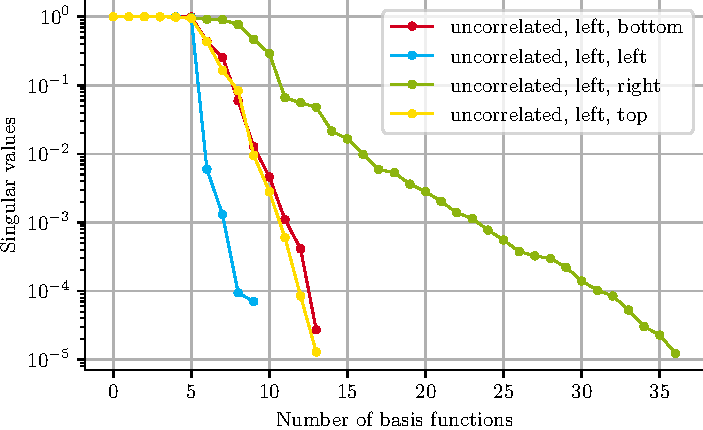
\includegraphics[width=0.6\textwidth]{../work/beam/fig_loc_svals_left.pdf}
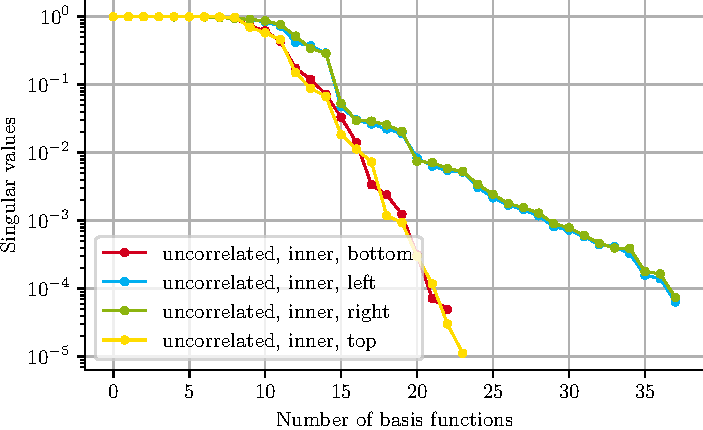
\includegraphics[width=0.6\textwidth]{../work/beam/fig_loc_svals_inner.pdf}
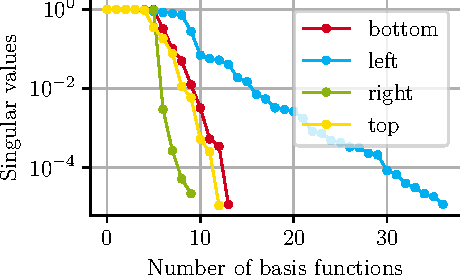
\includegraphics[width=0.6\textwidth]{../work/beam/fig_loc_svals_right.pdf}

\subsection{Projection Error}
The projection error is computed for a test set for each configuration that was computed
using the FOM. Each test set has size $n_{test}$.

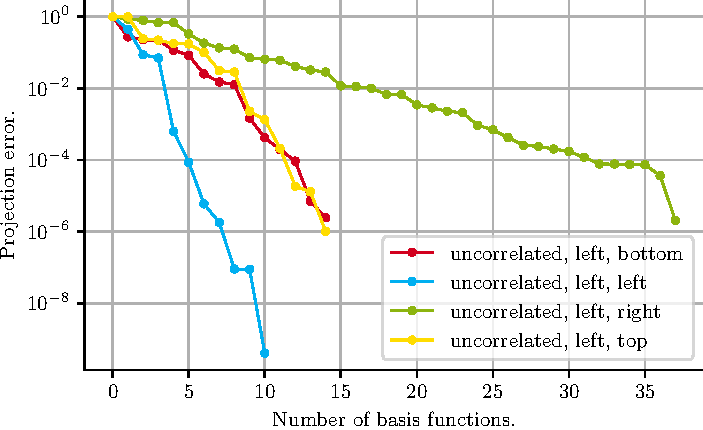
\includegraphics[width=0.6\textwidth]{../work/beam/fig_proj_error_left.pdf}
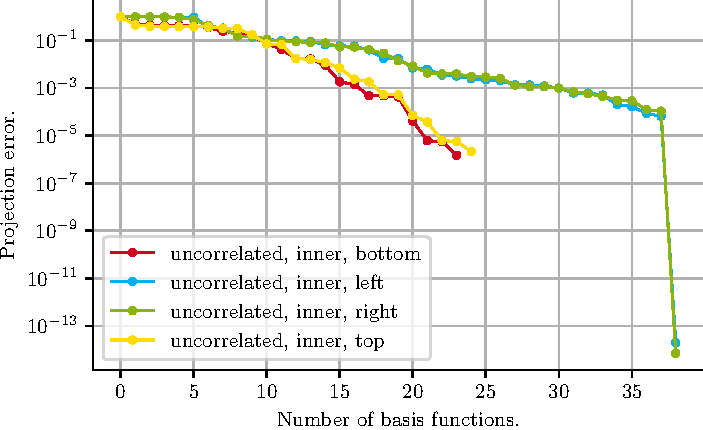
\includegraphics[width=0.6\textwidth]{../work/beam/fig_proj_error_inner.pdf}
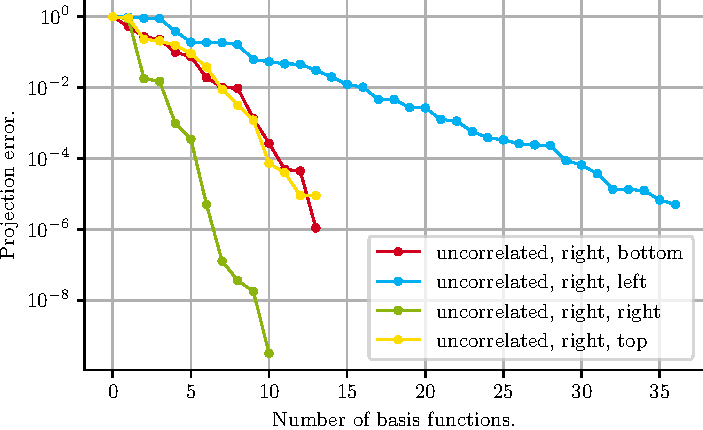
\includegraphics[width=0.6\textwidth]{../work/beam/fig_proj_error_right.pdf}

\section{Conclusions}

% TODO Bibliography
% TODO backmatter

\end{document}
